% !TeX root = ./CuckooSearch_roessig_rueckauf.tex
\documentclass[conference]{IEEEtran}
\IEEEoverridecommandlockouts
% The preceding line is only needed to identify funding in the first footnote. If that is unneeded, please comment it out.
\usepackage[ngerman]{babel}
\usepackage[utf8]{inputenc}
\usepackage{cite}
\usepackage{amsmath,amssymb,amsfonts}
\usepackage{algorithm}
\usepackage{algpseudocode}
\usepackage{graphicx}
\usepackage{textcomp}
\usepackage{xcolor}
\def\BibTeX{{\rm B\kern-.05em{\sc i\kern-.025em b}\kern-.08em
    T\kern-.1667em\lower.7ex\hbox{E}\kern-.125emX}}
\begin{document}

  \title{Anwendung des Cuckoo Search Algorithmus auf das Traveling Salesman und das Sequential Ordering Problem}

  \author{
    \IEEEauthorblockN{
      1\textsuperscript{st} Lennard Rössig}
      \IEEEauthorblockA{\textit{Hochschule Hannover} \\
      \textit{Fakultät IV - Abteilung Informatik}\\
              Hannover, Niedersachsen \\
              lennard.roessig@stud.hs-hannover.de}
    \and
      \IEEEauthorblockN{
        2\textsuperscript{nd} Florian Rückauf}
        \IEEEauthorblockA{\textit{Hochschule Hannover} \\
        \textit{Fakultät IV - Abteilung Informatik}\\
                Hannover, Niedersachsen \\
                florian.rueckauf@stud.hs-hannover.de}
  }

  \maketitle

  \begin{abstract}
    In dieser Arbeit wurde der metaheuristischen Algorithmus Cuckoo Search (CS) implementiert, um damit zwei Optimierungsproblem zu lösen. 
    Die grundlegende Idee des Algorithmus ist abgeleitet von dem Brutparasitismus einiger Kuckuck-Arten. Das Bewegungsmuster des Kuckucks 
    wird in dem Algorithmus durch den Levy Flight erzeugt. Dieser erzeugt ein Bewegungsmuster wie es bei einigen Vögeln und Insekten 
    beobachtet wurde.  Es wurden die beiden NP-harten Probleme, des Travelling-Salesmans (TSP) und des Sequenc-Ordering (SOP) betrachtet 
    und mit dem Algorihtmus gelöst. Da die Arbeit im Kontext eines Projektes erscheint, in dem mehrere metaheuristische Algorithmen verglichen 
    wurden, sind zum Schluss nur die Benchmarks und Ergebnisse des hier angewandten Algorithmus gelistet.
  \end{abstract}

  \begin{IEEEkeywords}
    algorithm; cuckoo search; Levy Flight; meta-heuritics; nature-inspired strategy; optimization
  \end{IEEEkeywords}

  \section{Einleitung}
    Viele Optimierungsprobleme sind NP-hart und damit existiert kein Algorithmus, der dieses Problem effizient lösen kann. Für solche 
    Probleme können Metaheuristiken zur näherungsweisen Lösung eingesetzt werden. Metaheuristiken definieren dabei eine abstrakte Folge 
    von Schritten, die auf beliebige Problemstellungen angewandt werden können. Die einzelnen Schritte müssen allerdings wieder 
    problemspezifisch implementiert werden. Erfolg und Laufzeit hängen von der Definition und Implementierung dieser Schritte ab. 

    Ein Bereich der Metaheuristiken sind die naturanalogenen Algorithmen, deren Vorgehen sich aus der Natur ableitet. In diesem Zusammenhang 
    wird der Cuckoo Search (CS) Algorithmus betrachtet und einmal auf das Traveling Salesman Problem (TSP) und Sequential Ordering Problem (SOP) 
    angewandt. Der CS ist ein noch recht junger Algorithmus, der 2009 von Xin-She Yang und Suash Deb entwickelt wurde \cite{b1}. 
    Die Experimente wurden für das euklidische, symmetrische TSP durchgeführt und die genutzten Daten stammen aus der TSPLIB Library \cite{b12}.

  \section{Traveling Salesman Problem und Sequential Ordering Problem}
    \subsection{Traveling Salesman Problem}
      Bei dem TSP wird ein Hamiltonkreis mit den minimalen Kosten $H_{opt}$ in einem vollständigen, 
      gewichteten Graphen $G = (V,E)$ gesucht \cite{b2}, \cite{b3}. Die Städte werden hier durch 
      die Knoten $V$ repräsentiert und die Verbindungen zwischen den Städten $u$ und $v$ sind die 
      Kanten $E = (u,v)$. Zu jeder Kante gibt es eine Länge $c_{u,v} \geq 0$. Da sich die Knoten hierbei 
      in dem zweidimensionalen euklidischen Raum befinden, handelt es sich um das euklidische TSP. 
      Die Länge $c_{u,v}$ ist somit für alle $u,v$ in $G$ die euklidische Entfernung zwischen den beiden Städten, 
      die den Knoten $u$ und $v$ zugeordnet sind. Betrachtet wurde das symetrische TSP, bei dem die Strecke 
      zwischen zwei Städten $c_{u,v}$ gleich der Strecke $c_{v,u}$ ist.


    \subsection{Sequential Ordering Problem}
      Beim Sequential Ordering Problem (SOP) handelt es sich wie beim TSP um einen Graphen im euklidischen zweidimensionalen Raum. 
      Im Gegensatz zum TSP sind die Eigenschaften einer korrekten (engl. valid) Reihenfolge strenger. Hierbei müssen 
      bestimmte Bedingungen (engl. Condition) hinsichtlich des Aufbaus einer solchen Reihenfolge eingehalten werden. 
      Ist $P$ die Menge aller Knoten des SOP's so lässt sich jeder Knoten mittels $P_i | i \in \mathbb{N}$ referenzieren. 
      Um eine korrekte Reihenfolge zu konstruieren, muss diese mit $P_0$ starten und auf $P_{n-1}$ enden. 
      Bei $P_0$ und $P_{n-1}$ handelt es sich um einen festen Start- und Endknoten. Der Endknoten ist dabei der letzte Knoten 
      des Problems, daher ist $n = |P|$.  Zusätzlich zu dieser Einschränkung besitzen die Knoten untereinander Beziehungen/Bedingungen. 
      Eine Bedingung bedeutet, dass ein bestimmter Knoten vor einem anderen Knoten in der Reihenfolge liegt. Besitzt also $P_x$ eine 
      Bedingung zu $P_y$ so muss $P_y$ vor $P_x$ in der Reihenfolge besucht werden. Jeder Knoten besitzt eine Bedingungsmenge $B_i | i \in \mathbb{N}$, 
      wobei $i$ die Bedingungsmenge des $i$-ten Knotens des Problems $P$ meint. Für eine korrekte Reihenfolge müssen also folgende Bedingungen gelten:
      \begin{itemize}
        \item jeder Knoten wird nur einmal besucht
        \item alle Bedingungen werden eingehalten
      \end{itemize}
    
      In den Bedingungen lassen sich die festen Start- und Endknoten definieren. 
      Die Bedingungsmenge des Startknotens \eqref{Bedingungsmenge P0} ist leer, 
      da dieser ganz vorne stehen muss. Im Gegensatz enthält die Bedingungsmenge des 
      Endknotens \eqref{Bedingungsmenge Pn} alle anderen Knoten, da diese vor ihm sein müssen. 
    
      
      \begin{equation}\label{Bedingungsmenge P0}
          B_0 = \emptyset
      \end{equation}
    
      
      \begin{equation}\label{Bedingungsmenge Pn}
          B_{n-1} = P\backslash\{P_{n-1}\}
      \end{equation}
    
      Für die Bedingungen gilt zusätzlich, dass ein Knoten nicht zu sich selber eine Bedingung besitzen kann.
      Des Weiteren kann ein Knoten aber nicht eine Bedingung zu einem anderen Knoten besitzen, wenn dieser eine Bedingung zu ihm hat. 
      Falls eine solche Beziehung erlaubt wäre, wäre das SOP unlösbar, da beide Knoten jeweils den anderen Knoten vor sich erwarten.
      Die Bedingungsmenge alle andere Knoten \eqref{Bedingungsmenge Pi} darf nicht sich selbst und den Endknoten enthalten, aber muss den Startknoten
      besitzen.

      \begin{equation}\label{Bedingungsmenge Pi}
          B_i \subseteq P\backslash\{P_i, P_n\} | B_i \cap \{P_0\} \neq \emptyset
      \end{equation}


  \section{Grundlagen des Cuckoo Search}
    \subsection{Brutverhalten des Kuckucks}
      Die Grundidee des Algorithmus wurde von dem Brutverhalten des namensgebenden Kuckucks abgeleitet. Das Brutverhalten des Kuckucks 
      ist der sogenannter Brutparasitismus. Bei diesem Verhalten wird das eigene Gelege nicht selbst bebrütet, sondern es wird ein 
      Ersatzwirt gesucht, der das Ei ausbrütet und sich auch um die Fütterung und Aufzucht des fremden Nachwuchses kümmert.

      Die Brutschmarotzer müssen sich durch dieses Verhalten nicht um die zeitintensive Aufzucht der Nachkommen kümmern. 
      Sie verringern somit den Aufwand für die Brutpflege und haben mehr Zeit Nahrung für sich selbst zu finden. Dadurch sind 
      sie in der Lage mehr Eier zu legen und können so potenziell mehr Nachkommen erzeugen. 

      Unter den Wirtstieren gibt es aber auch solche, die die fremden Eier entdecken. Dann gibt es zwei verschiedene Strategien. 
      Werden die fremden Eier entdeckt, so werden sie entweder aus dem Nest geschmissen oder das ganze Gelege wird verlassen und 
      ein neues angelegt. 

      Gerade in dem interspezifischen Brutparasitismus haben sich verschiedene Anpassungen entwickelt, um das Risiko der Entdeckung 
      zu minimieren. Bei einigen Arten erfolgt die Eireifung simultan zu der des Wirtstieres. Die Eier des Kuckucks besitzen meist 
      eine kürzere Brutzeit, sodass der Kuckuck als erster schlüpft und er dann die anderen Eier aus dem Nest schmeißt. Die meisten 
      Kuckucksküken wachsen in den ersten Tagen schneller als die Küken der Wirtseltern und haben dadurch einen entscheidenden 
      Fütterungs- und Wachstumsvorteil.  Zudem erfolgt die Eiablage in beschleunigter Form, d.h. das Ei wird im Eileiter aufbewahrt 
      und kann dann im Gelegenheitsfall schnell gelegt werden. Es wurden in der Natur Eiablagezeiten von nur 10 Sekunden gemessen. 
      Manche Kuckucksarten haben die Größe und Farbe der Eier denen der Wirtseier angepasst, sodass fast kein Unterschied zwischen 
      den Eiern mehr zu erkennen ist. Diese Tiere bevorzugen dann in der Regel eine Wirtsvogelart.         


    \subsection{Basis Version}
      Das oben beschriebene Verhalten wird in dem Cuckoo Search genutzt, um den Suchraum nach einer optimalen Lösung 
      zu durchsuchen. Der Algorithmus funktioniert dabei wie folgt \cite{b1}:

      \begin{itemize}
        \item Ein Set von Nestern mit einem Ei wird zufällig in dem Suchraum platziert. Die Anzahl der Nester 
          ist dabei fest und ändert sich im Laufe des Algorithmus nicht. 

        \item Eine Anzahl von Kuckucken durchfliegt den Suchraum und generiert damit eine neue Lösung. Diese 
          neue Lösung wird in ein zufällig gewähltes Nest gelegt. 

          In diesem Szenario repräsentiert jedes Ei in einem Nest eine Lösung und jeder Kuckuck repräsentiert eine 
          neue Lösung. Das Ziel ist es, die neuen, potenziell besseren Lösungen zu nehmen und damit eine andere, 
          nicht so gut Lösung aus dem Nest zu verdrängen. 

        \item Die Wahrscheinlichkeit, dass ein Ei durch den Wirt entdeckt wird, liegt dabei in dem Bereich $p_{a}[0,1]$. 
          Tritt dieser Fall ein, so wird entweder das Ei aus dem Nest geschmissen oder das ganze Nest wird verlassen 
          und ein neues wird gebaut. Für die Einfachheit wird die letztere Möglichkeit angenommen, d.h. mit 
          der Wahrscheinlichkeit von $p_{a}$ werden $n$ Nester durch neue Nester ersetzt, die eine neue, zufällige Lösung besitzen. 
      \end{itemize}

      Die besten Nester mit den besten Lösungen werden dann genutzt, um daraus neue Generationen zu erzeugen. 
      Der Algorithmus kann noch dahin geändert werden, dass ein Nest mehrere Eier enthält und somit eine Menge an Lösungen beinhaltet.

      {Algorithm \ref{cuckooSearch}} zeigt den Pseudo Code für den Cuckoo Search. 

      \begin{algorithm}
      \caption{Cuckoo Search}\label{cuckooSearch}
        \begin{algorithmic}[1]
        \State Objective function $f(x), x = (x_{i}, ...,x_{d})^T$
        \State Generate initial population of $n$ host nests $x_{i} (i =1,...,n)$
        \While{($t <$ MaxGeneration) or (stop criterion)}
          \State Get a cuckoo randomly by Lévy Flights
          \State Evaluate its quality/fitness $F_{i}$
          \State Choose a nest among $n$ (say, $j$) randomly
          \If {$F_{i} > F_{j}$} 
            \State replace $j$ by the new solution
          \EndIf
          \State A fraction $(p_{a})$ of worse nest are abandoned 
          \State and new ones are buildt 
          \State Keep the best solutions (or nest with quality solutions)
          \State Rank the solutions an find the current best
        \EndWhile
        \State Postprocess results and visualization
        \end{algorithmic}
      \end{algorithm}

      Um eine neue Generation von Lösungen von einem Kuckuck zu erzeugen, wird der Lévy Flight genutzt. 
      In verschiedenen Studien wurde gezeigt, dass das Flugverhalten verschiedener Tiere und Insekten die 
      Eigenschaft eines Lévy Flights besitzen \cite{b4},\cite{b5},\cite{b6}. Die Definition des Lévy Flights 
      stammt von Mathematikern der Chaostheorie und ist sehr nützlich, um zufällige oder pseudo-zufällige natürliche 
      Phänomena zu beschreiben. Abbildung \ref{fig:levyFlight} zeigt ein Beispiel eines Lévy Flights beginnend im Punkt (0,0).

      \begin{figure}
        \centering
        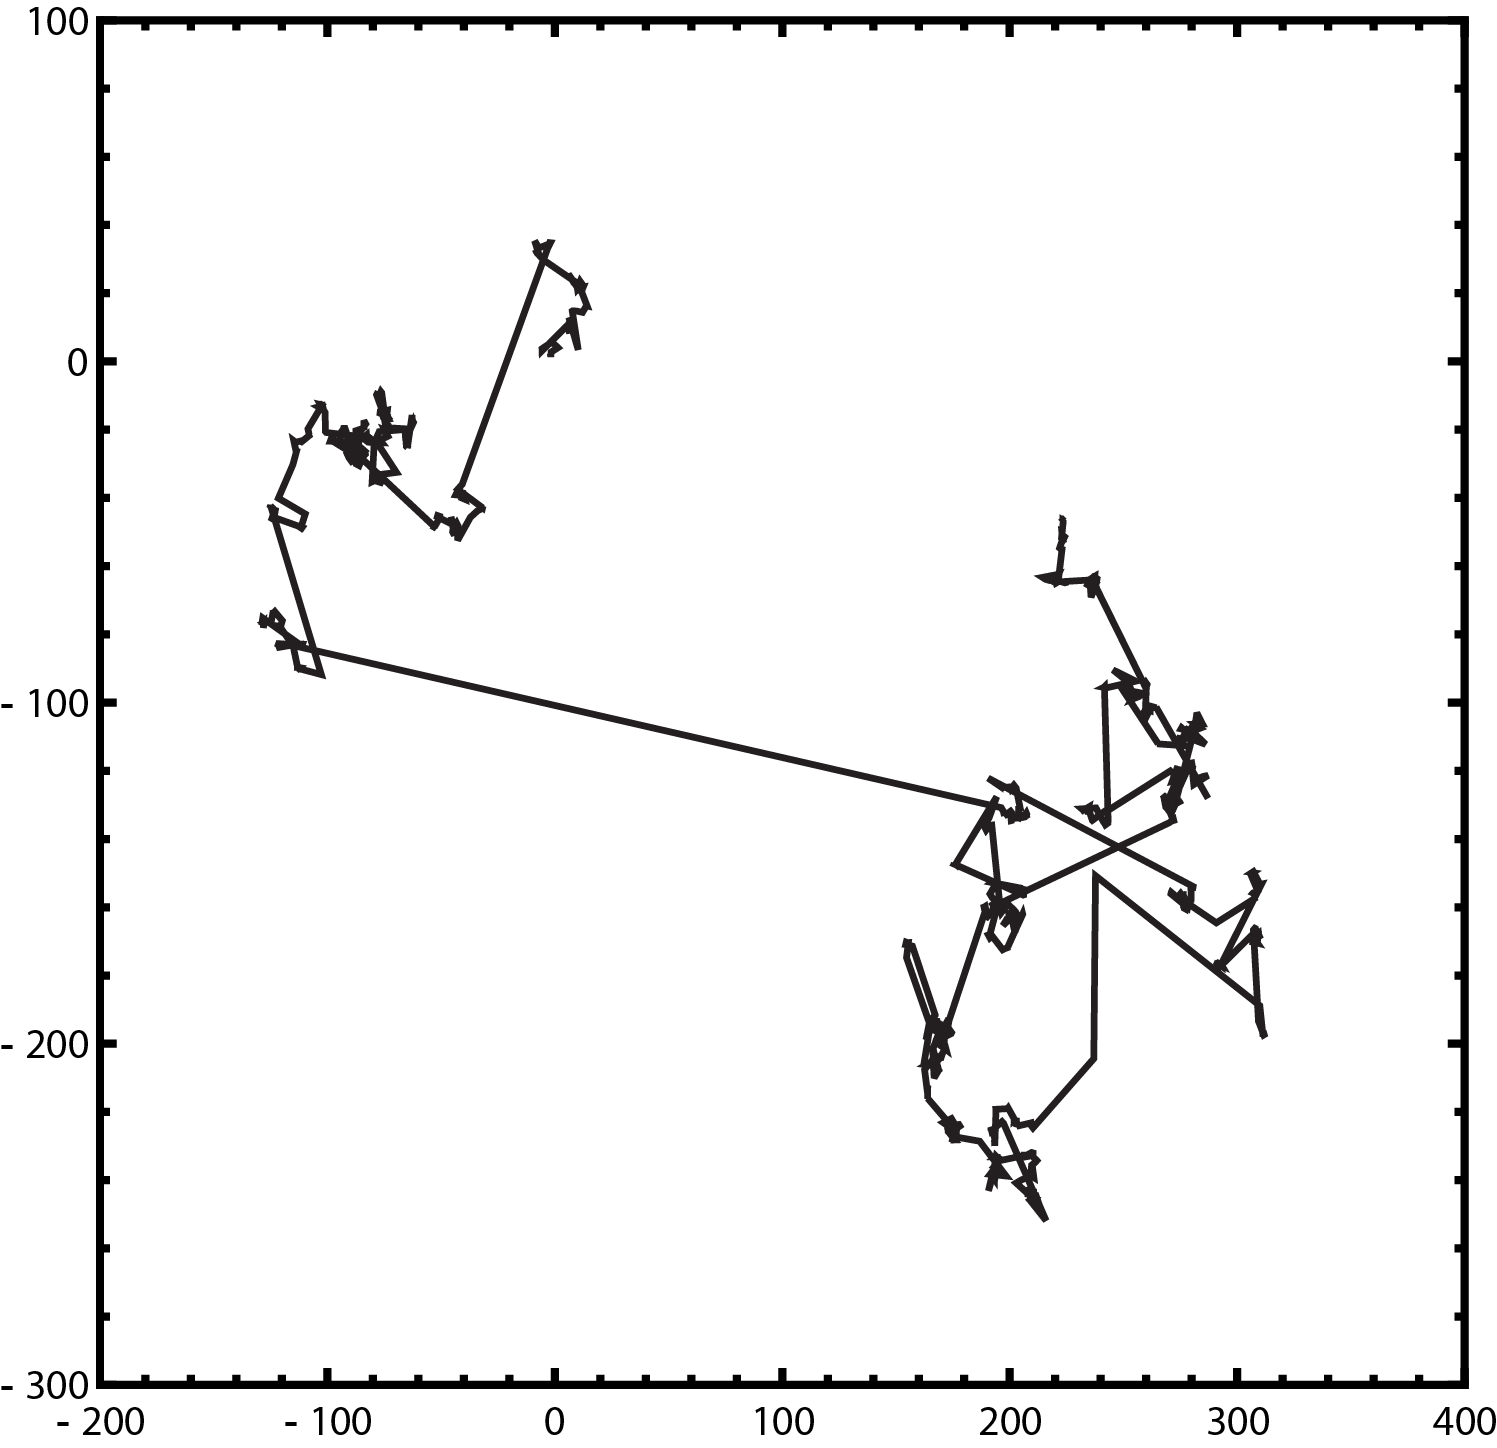
\includegraphics[width=0.8\linewidth]{LevyFlight.png}
        \caption{Lévy Flight beginnend im Punkt (0,0).}
        \label{fig:levyFlight}
      \end{figure}


      Die Erzeugung einer neuen Lösung über den Lévy Flight wird mit der Gleichung

      \begin{equation}
      x_{i}^{t+1} = x_{i}^{t} + \alpha L(s, \lambda)\label{eq}
      \end{equation}

      beschrieben. Der Parameter $\alpha > 0$ beschreibt den Skalierungsfaktor der Schrittweite.  
      In \cite{b7} wird $\alpha$ durch $\alpha = O(L/10)$ berechnet. Bei Problemen in denen verhindert 
      werden soll, das zu weit geflogen wird, kann $\alpha = O(L/100)$ genutzt werden. $L$ ist dabei die 
      Skalierung für das spezifische Problem.

      Um den Lévy Flight zu implementieren ist ein schneller Algorithmus nötig, der den Lévy Flight approximiert. 
      In \cite{b8} werden drei Algorithmen für die Approximation des Lévy Flights verglichen. Der 
      Mantegna Algorithmus benötigt für die Aufgabe die unten aufgeführten drei Schritte. Die Schrittweite $s$ wird mit
      
      \begin{equation}
        s = \frac{u}{|v|^{\frac{1}{\beta}}}\label{eq}
      \end{equation}

      berechnet, wobei $u$ und $v$ durch die Normalverteilung

      \begin{equation}
        u = N(o,\sigma_{u}^{2}), v = N(o,\sigma_{v}^{2})\label{eq}
      \end{equation}

        gegeben sind. Die Varianz $\sigma$ wird dabei mit

      \begin{equation}
        \sigma_{u} = \left(\frac{\Gamma(1 + \beta)\sin(\pi\beta/2)}{\Gamma[(1 + \beta)/2)]\beta2^{(\beta-1)/2}}\right)^{\frac{1}{\beta}} , \sigma_{v} = 1 \label{eq}
      \end{equation}

      berechnet, wobei $1 \leq \beta \leq 2$ und $\Gamma$ die Gammafunktion ist. 

    \subsection{Verbesserte Version}
      In der Basisversion wird noch nicht das unterschiedliche Verhalten der Kuckucke bei der Auswahl 
      des Nests in betracht gezogen. Quaarrad et al. \cite{b9} beschreibt eine Möglichkeit die Art und 
      Weise, wie ein Kuckuck den Suchraum erkundet, zu verbessern. Ein Kuckuck kann eine gewisse Intelligenz 
      besitzen, so dass er bessere Lösungen findet. Dadurch kann die Intensivierung und die Diversifikation der 
      Suche durch den Kuckuck beeinflusst werden. Angepasst an das intelligenter Verhalten einiger Kuckucke, 
      führt ein Teil der Kuckucke einen initialen Schritt zu einer neuen Lösung über 
      den Lévy Flight durch und suchen von dort aus eine neue, bessere Lösung über eine lokale Suche.

      Ausgehend davon, kann die Population der Kuckucke in dem verbesserten CS in drei Typen unterteilt werden.

      \begin{enumerate}
        \item Der Kuckuck sucht von der besten Position aus neue Gebiete welche besser Lösung beinhalten können, durch eine zufällige Auswahl.
        \item Ein Teil $p_{a}$ der Kuckucke sucht eine Lösung weit weg von der besten Lösung
        \item Ein Teil $p_{c}$ der Kuckucke sucht nach Lösungen von der aktuellen Position und versucht diese zu 
          verbessern. Sie bewegen sich von einer Region zu einer anderen durch den Lévy Flight um die beste Lösung 
          in jeder Region zu bekommen, ohne in einem lokalen Minimum festsitzen zu bleiben.
      \end{enumerate}

      Diese Anpassungen verbessern die Intensität der Suche um die aktuell besten Lösungen und gleichzeitig wird 
      die Zufälligkeit mit der neue Gebiete erschlossen werden erhöht. Dadurch wird die Performanz und die Effizienz 
      verbessert, da weniger Iterationen benötigt werden und er eine besser Resistenz gegenüber lokalen Minima besitzt \cite{b9}.

  \section{Anpassung des Cuckoo Search für die betrachteten Probleme}
    \subsection{Cuckoo Search für das Traveling Salesman Problem}
      Bekanntlich befindet sich das TSP in einem kombinatorischen Raum. Der CS wurde entworfen, 
      um Lösungen in einem kontinuierlichen Raum zu finden. Um jetzt den CS für die Lösung des TSP anzupassen, 
      müssen die fünf Hauptbegriffe des CS (Ei, Nest, Zielfunktion, Suchraum und Lévy Flight) an das TSP angepasst werden. 

      Im CS repräsentiert ein Ei eine möglich Lösung das Problems. Beim TSP ist eine mögliche Lösung eine 
      Route durch alle Städte. Diese Route ist ein Hamiltonkreis.

      Ein Nest enthält die Eier, also enthält ein Nest ein oder mehrere mögliche Lösungen des Problems. 
      In diesem Fall also ein oder mehrere Hamiltonkreise.

      Beim TSP ist die kürzeste Route zwischen den Städten gesucht. Als Zielfunktion wird hier 
      die Länge des Hamiltonkreises genutzt. 

      Da die Positionen der Städte fest sind und diese nicht verändert werden können, lässt sich 
      die Lösungen nur durch die Reihenfolge der besuchten Städte verändern. Der Suchraum umfasst somit alle 
      möglichen Anordnungen der Städte. Die Reihenfolge der besuchten Städte lässt sich mit dem 2-opt-move \cite{b10} 
      und den Double-Bridge-move \cite{b10} verändern. Der 2-opt-move wird dabei genutzt, um eine kleine Änderung 
      in dem Suchraum zu erzeugen und der Double-Bride-move wird für große Änderungen genutzt. Wie 
      in Abbildung \ref{fig:2-opt-move} zu sehen, entfernt der 2-opt-move zwei Kanten und erstellt zwei neue Kanten. 
      Der Double-Bride-move entfernt vier Kanten und erstellt neue Kanten, so wie in 
      Abbildung \ref{fig:double-bridge-move} zu sehen ist.

      \begin{figure}
      \centering
        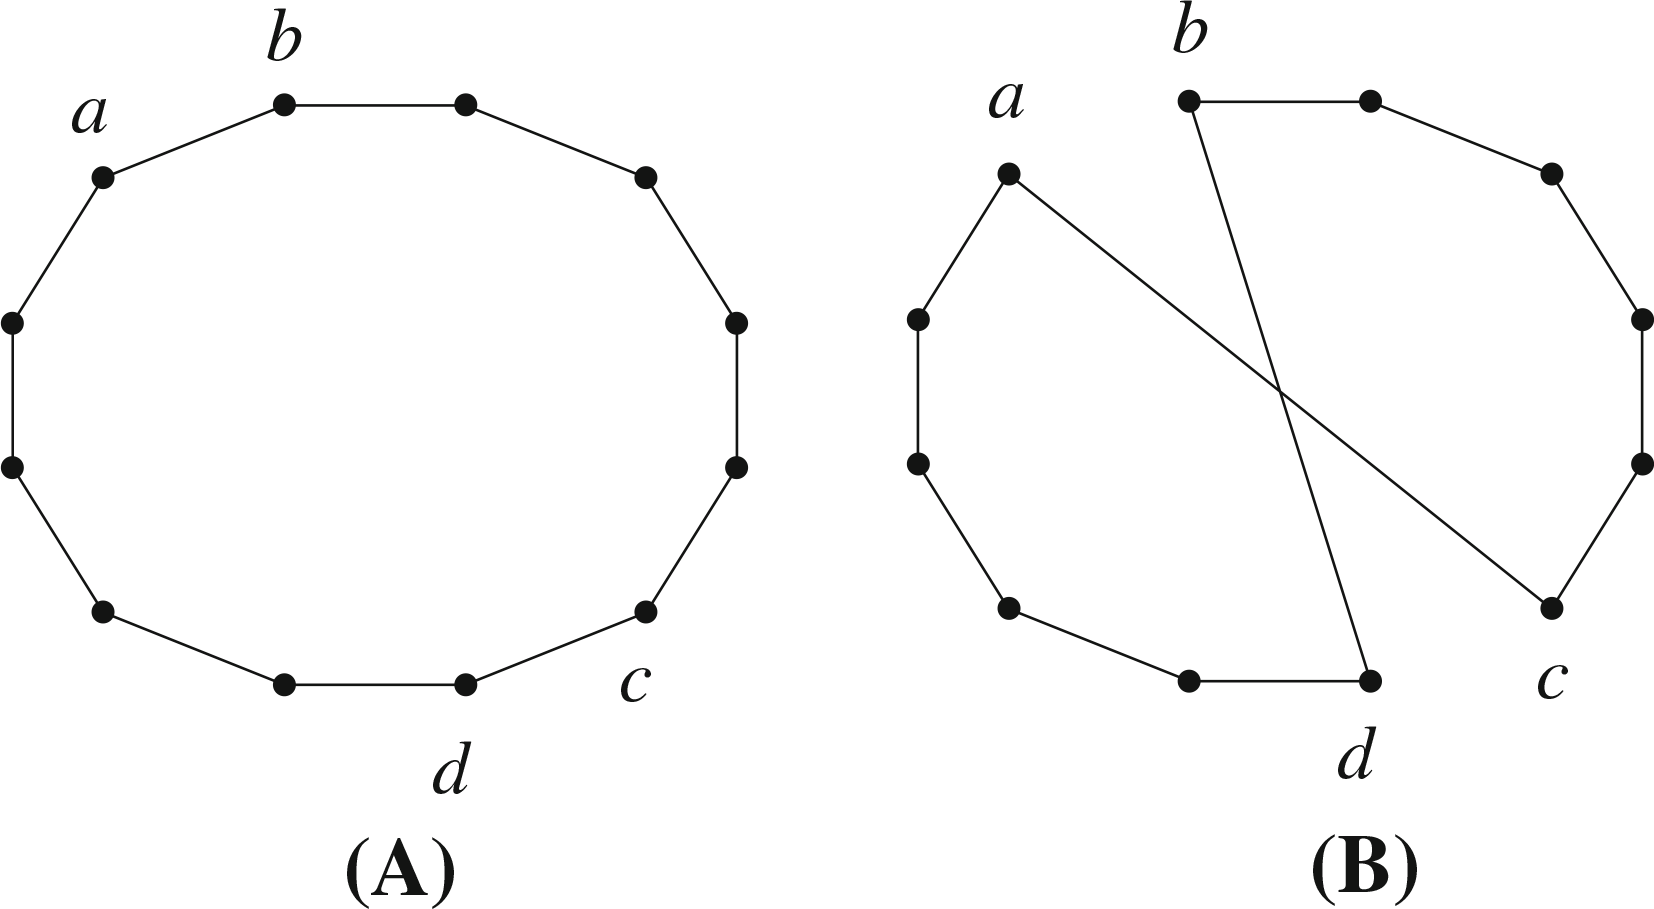
\includegraphics[width=0.8\linewidth]{2-opt-move.png}
        \caption{2-opt-move. a initiale Tour. b durch 2-opt-move erzeugte Tour. Kanten (a,b) und (d,c) wurden durch Kanten (a,c) und (b,d) ersetzt}
        \label{fig:2-opt-move}
      \end{figure}

      \begin{figure}
      \centering
        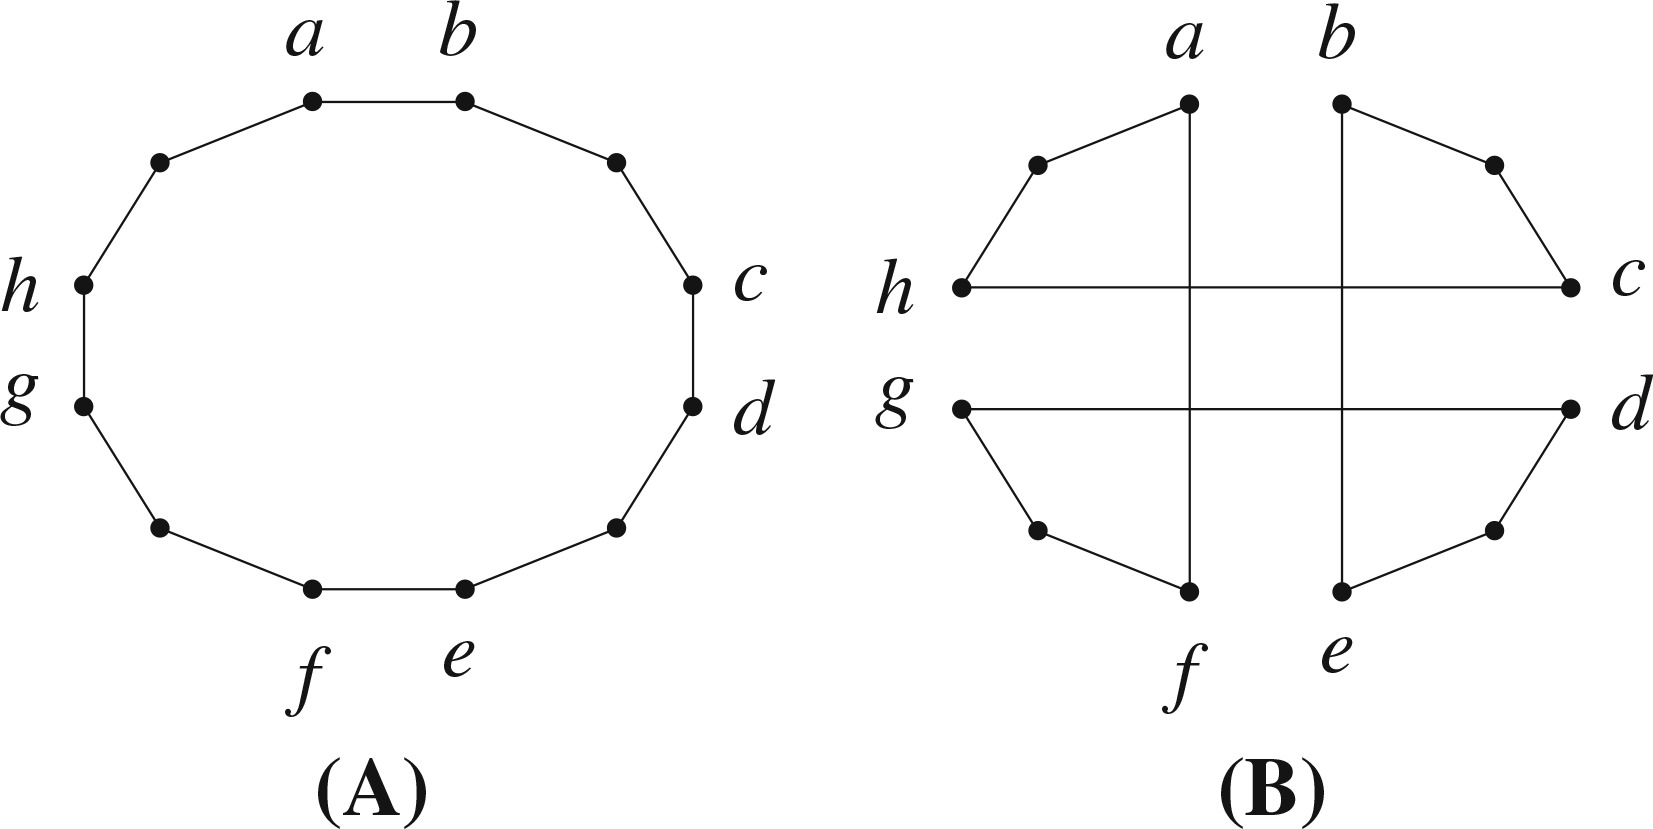
\includegraphics[width=0.8\linewidth]{double-Bridge.png}
        \caption{Double-Bridge-move. a initiale Tour. b durch Double-Bridge-move erzeugte Tour. Kanten 
        (a,b), (c,d), (e,f) und (g,h) wurden durch Kanten (a,f), (g,d), (e,b) und (g,d) ersetzt}
        \label{fig:double-bridge-move}
      \end{figure}

      Um den Suchraum zu durchsuchen, haben wir die Möglichkeit dies in kleinen Schritten, 
      oder in großen Schritten zu tun. Um jetzt die Schrittweise an den Lévy Flight anzupassen, 
      werden die Werte des Lévy Flight auf ein Intervall zwischen 0 und 1 abgebildet. Das Intervall kann dann in 
      verschiedene Abschnitte unterteilt werden, so dass wir die Schrittlänge anpassen können.
      Je nach Wert des Lévy Flight ergibt sich dann die Schrittweite nach
      \begin{enumerate}
        \item$[0,i[$ ein Schritt durch 2-opt-move
        \item$[(k-1)*i, k*i[$ $k$ Schritte durch $k * 2-opt-move$
        \item$[k*i,1[$ ein großer Schritt durch double-bridge-move
      \end{enumerate}


    \subsection{Cuckoo Search für das Sequential Ordering Problem}
      Der größte Unterschied für den Cuckoo-Algorithmus vom TSP zum SOP ist, dass der Algorithmus Lösungen 
      produzieren kann die nicht mehr korrekt (engl. valid) sind. Für das TSP wurden nur korrekte Lösungen erstellt, wenn die 
      Operatoren auf korrekten Reihenfolgen arbeiten. Daher ist es ausreichend dort, darauf zu achten, dass die Initialisierung 
      nur korrekt Reihenfolge erbrachte. Anschließend konnte durch die Operaten die Double-Bridge-move 
      \ref{fig:double-bridge-move} und 2-opt-move \ref{fig:2-opt-move} keine inkorrekten Ergebnisse erzeugt werden.
      Mit SOP reicht es nicht mehr nur die Initialisierung korrekt zu gestalten, da auch die 
      beiden Operationen zu inkorrekt Ergebnissen führen können.
      Im folgenden werden drei Varianten vorgestellt, die den Umgang mit inkorrekten Reihenfolge auf unterschiedliche
      Art lösen. Anschließend wird die Implementierung einer dieser Varianten für den Cuckoo's Algorithmus gezeigt. 

    \subsection{Handicap}
      Beim Handicap werden invalide 
      Ergebnisse in der Population beibehalten. Ihre Fitness hingegen wird mittels eines Handicaps 
      verschlechtert. Das Abschwächen ist die ''Bestrafung'' dafür das es sich bei der 
      Lösung um ein invalides Ergebnis handelt. Der Vorteil dieser Variante ist, dass auch eine solche 
      Lösung noch gute Bestandteile beinhalten kann, die vom Schwarm noch sinnvoll übernommen werden können. 
      Besitzen diese aber keine guten Bestandteile, verschlechtern sie sich durch das Handicap stark, sodass diese aus der
      Population ausscheiden. Nachteil an diesem Ansatz ist, dass das Balancing des Handicaps 
      enorm schwer ist. Ist das Handicap viel zu stark, werden invalide Lösung nicht wirklich 
      betrachten und könnten auch direkt gelöscht werden. Ist wiederrum das Handicap zu schwach, 
      kann es passieren, dass die beste Lösung des Algorithmus ein invalides Ergebnis ist, was 
      wiederrum unerwünscht ist. Erst recht ist das Handicap im Falle von SOP/TSP schwer 
      einzubringen, da die Fitness hierbei die Länge der Pfade ist. Die Problemstellung äußert 
      sich also direkt in der Fitness was wiederrum bedeutet, dass eine Fitness von 100 in dem einem Fall
      gut und in einem anderen Fall schlecht ist. Das Handicap müsste daher variable gestaltet werden. Problem hierbei ist, dass das optimale Ergebnis zu Beginn nicht 
      bekannt ist, wodurch ein relatives Handicap schwer umzusetzen ist. Des Weiteren besitzt der Cuckoo's Algorithmus
      nicht das klassische Verhalten eines Schwarms, da die einzelnen Individuen sich nicht stark aneinander Orientieren.
      Aufgrund des fehlenden Schwarm-Verhaltens, dem Balancing und dem Problem des schwer an zu passenden Handicaps, 
      haben wir uns gegen diese Methode entschieden.

    \subsection{Operatoren} 
      Eine weitere Variante ist es, die Operatoren \textit{Double-Bridge-Move} und \textit{2-opt-swap} soweit anzupassen, dass diese
      nur noch korrekte Ergebnisse erzeugen. Die beiden Operatoren des Cuckoo's Algorithmus besitzen eine einfache 
      Struktur ohne weitere Metriken, wodurch eine solche Veränderung schwer ist. 
      Des Weiteren würde eine solche Anpassung die Komplexität der Operatoren erhöhen, wodurch die Grundidee eines 
      einfach zu verstehenden Optimierungsalgorithmus verloren gehen würde. 
      Grad die Einfachheit des Cuckoo's Algorithmus macht diesen aus, weshalb wir uns gegen diese Anpassung entschieden haben.


    \subsection{Reparierung}
      Im Repair-Schritt wird ein ungültiger Weg wieder in einem gültigen Weg transformiert, wobei 
      versucht wird den gültigen Wissensgehalt, innerhalb der Lösung, nicht zu verändern. Dies bedeutet, 
      dass gerade so viel geändert wird, dass die Reihenfolge wieder korrekt ist. Veränderungen darüber hinaus, 
      könnte dazu führen, dass kleiner Veränderungen durch die Operanten sonst verloren gehen würden.
      Des Weiteren ist der \textit{Repair-Schritt} ein unnatürlicher Eingriff in die natürliche Lösungsfindung des Cuckoo's Algorithmus, 
      weswegen dieser möglichst klein ausfallen sollte.
      Der \textit{Rapair-Schritt} schien uns für den Cuckoo's Algorithmus am passendsten, da dieser die Komplexität des Algorithmus nicht erhöht, aber 
      gleichzeitig keine weiteren Probleme mit sich bringt. 
      Die genaue Implementierung des Schrittes wird im folgenden Abschnitt beschrieben.


    \subsection{Implementierung} \label{Implementierung Repair}
      Im Cuckoo's Algorithmus, muss an drei Orten festgestellt werden, dass nur korrekte Reihenfolgen erstellt werden. 
      Die einzigen Punkte im Algorithmus wo inkorrekte Ergebnisse auftreten können, ist bei der \textit{Initialisierung} 
      und nach den beiden Operatoren. Da die \textit{Initialisierung} TSP Reihenfolgen erstellt, werden diese im Nachhinein so 
      transformiert, dass sie dem SOP entsprechen. Der \textit{Two-Opt-Swap} kann zu invaliden Reihenfolgen führen, muss dies aber 
      nicht. Daher muss nach jeder Ausführung geprüft werden, ob es sich noch um eine valide Reihenfolge handelt. 
      Ausnahme ist hierbei, dass wenn mehrere \textit{Two-Opt-Swaps} hintereinander ausgeführt werden, nur das letzte Ergebnis 
      wieder zu einem validen transformiert wird. Dies folgt wieder dem Prinzip, dass nur möglichst wenig verändert/eingegriffen 
      werden soll. Der \textit{Double-Bridge-Move} führt immer zu einer invaliden Reihenfolge, dies folgt aus der Definition der Methode. 
      Daher wird hier nach jeder Durchführung die Reihenfolge wieder repariert. Der Ablauf des \textit{Repair-Schrittes} ist immer 
      der gleiche und wird im Pseudocode \ref{Alg.1.Repair} dargestellt.


      
      \begin{algorithm}
        \caption{Repair}\label{Alg.1.Repair}
        \begin{algorithmic}[1]
        \State Erhalte Reihenfolge $R$ mit Länge $n$
        \While{($i <$ $n$)}
          \State $y = i+1$
          \State $B_i$ ist die Bedingungsmenge des Knoten $i$
          \While{($y <$ $n$)}
            \If{$B_i \cap \{P_y\} \neq \emptyset$}
              \State tausche Knote $i$ mit Knoten $y$
              \State breche innere Schleife ab
            \EndIf
          \EndWhile
          \State Erhöhe $i+1$, falls innere Schleife nicht abgebrochen
        \EndWhile
        \State Valide Reihenfolge $R$
        
        \end{algorithmic}
        \end{algorithm}

      Die Laufzeit vom \textit{Repair-Schritt} beträgt dabei O($n^2$), wobei $n$ die Länge der Reihenfolge $R$ ist. Dies ergibt sich aus der Tatsache, dass
      jede $swap$-Operation wieder zu einer neuen Verletzung der Bedingungen führen kann, weswegen ab Stelle $i$ erneut begonnen wird.
      Um also alle möglichen Verletzungen der Bedingungen zu finden, muss jeder Knoten $n_1$ mit jedem nachfolgendem Knoten $n_2$ geprüft werden. 
      Wie oben beschrieben, ist die Laufzeit abhängig von der Länge der Reihenfolge und dadurch direkt auch von der Größe des SOP's. 
      Durch diese Abhängigkeit, die zuvor nicht bestand, wird die Auswertungen von großen SOP's erheblich langsamer.
  


  \section{Evaluierung}
    In diesem Abschnitt gehen wir auf die Parameter des Cuckoo's Algorithmus ein und prüfen ihren Einfluss auf die Qualität des Ergebnisses.
    Dabei untersuchen wir verschiedene Anzahlen an Nester und Iterationen sowie unterschiedliche Wahrscheinlichkeiten $P_a$ dafür, dass ein Ei entdeckt wird 
    und aus dem Nest geworfen wird. Die Ergebnisse werden anschließend genutzt um den Cuckoo's Algorithmus auf mehreren 
    Datensätzen zu testen.


    \subsection{Parameter}
      Alle Durchgeführten Tests arbeiten dabei auf dem Datensatz \emph{a280.tsp} der 280 Knoten besitzt. 
      Beginnen tun wir mit dem Parameter $P_a$, dieser beschreibt die Entdeckungswahrscheinlichkeit eines Eies und somit das Ausscheiden aus der Population. 
      Dafür haben wir den Algorithmus mit fünf unterschiedlichen Werten laufen lassen, wobei diese von 10\% bis zu 30\% reichen. 
      Die Anzahl der Nester lag bei 50 und die Generationen bei 1000. 
      Anhand der Ergebnisse (Abb \ref{fig:pa}) lässt sich erkennen, dass der Einfluss des Parameters auf die Güte der Lösung sehr gering ist. Eine 
      niedrigere Entdeckungswahrscheinlichkeit sorgt geringfügig für ein schnelleres Anpassungsverhalten, hingegen sich dies im Endergebnis nicht wiederspiegelt. 
      Für ein gutes Anpassungsverhalten sollte $P_a$ daher nicht zu niedrig gesetzt werden, aber auch nicht zu hoch, damit noch eine Anpassung stattfindet. 
      Die weiteren Tests werden daher mit einer $P_a = 0.15$ durchgeführt.

      \begin{figure}[H]
        \centering
        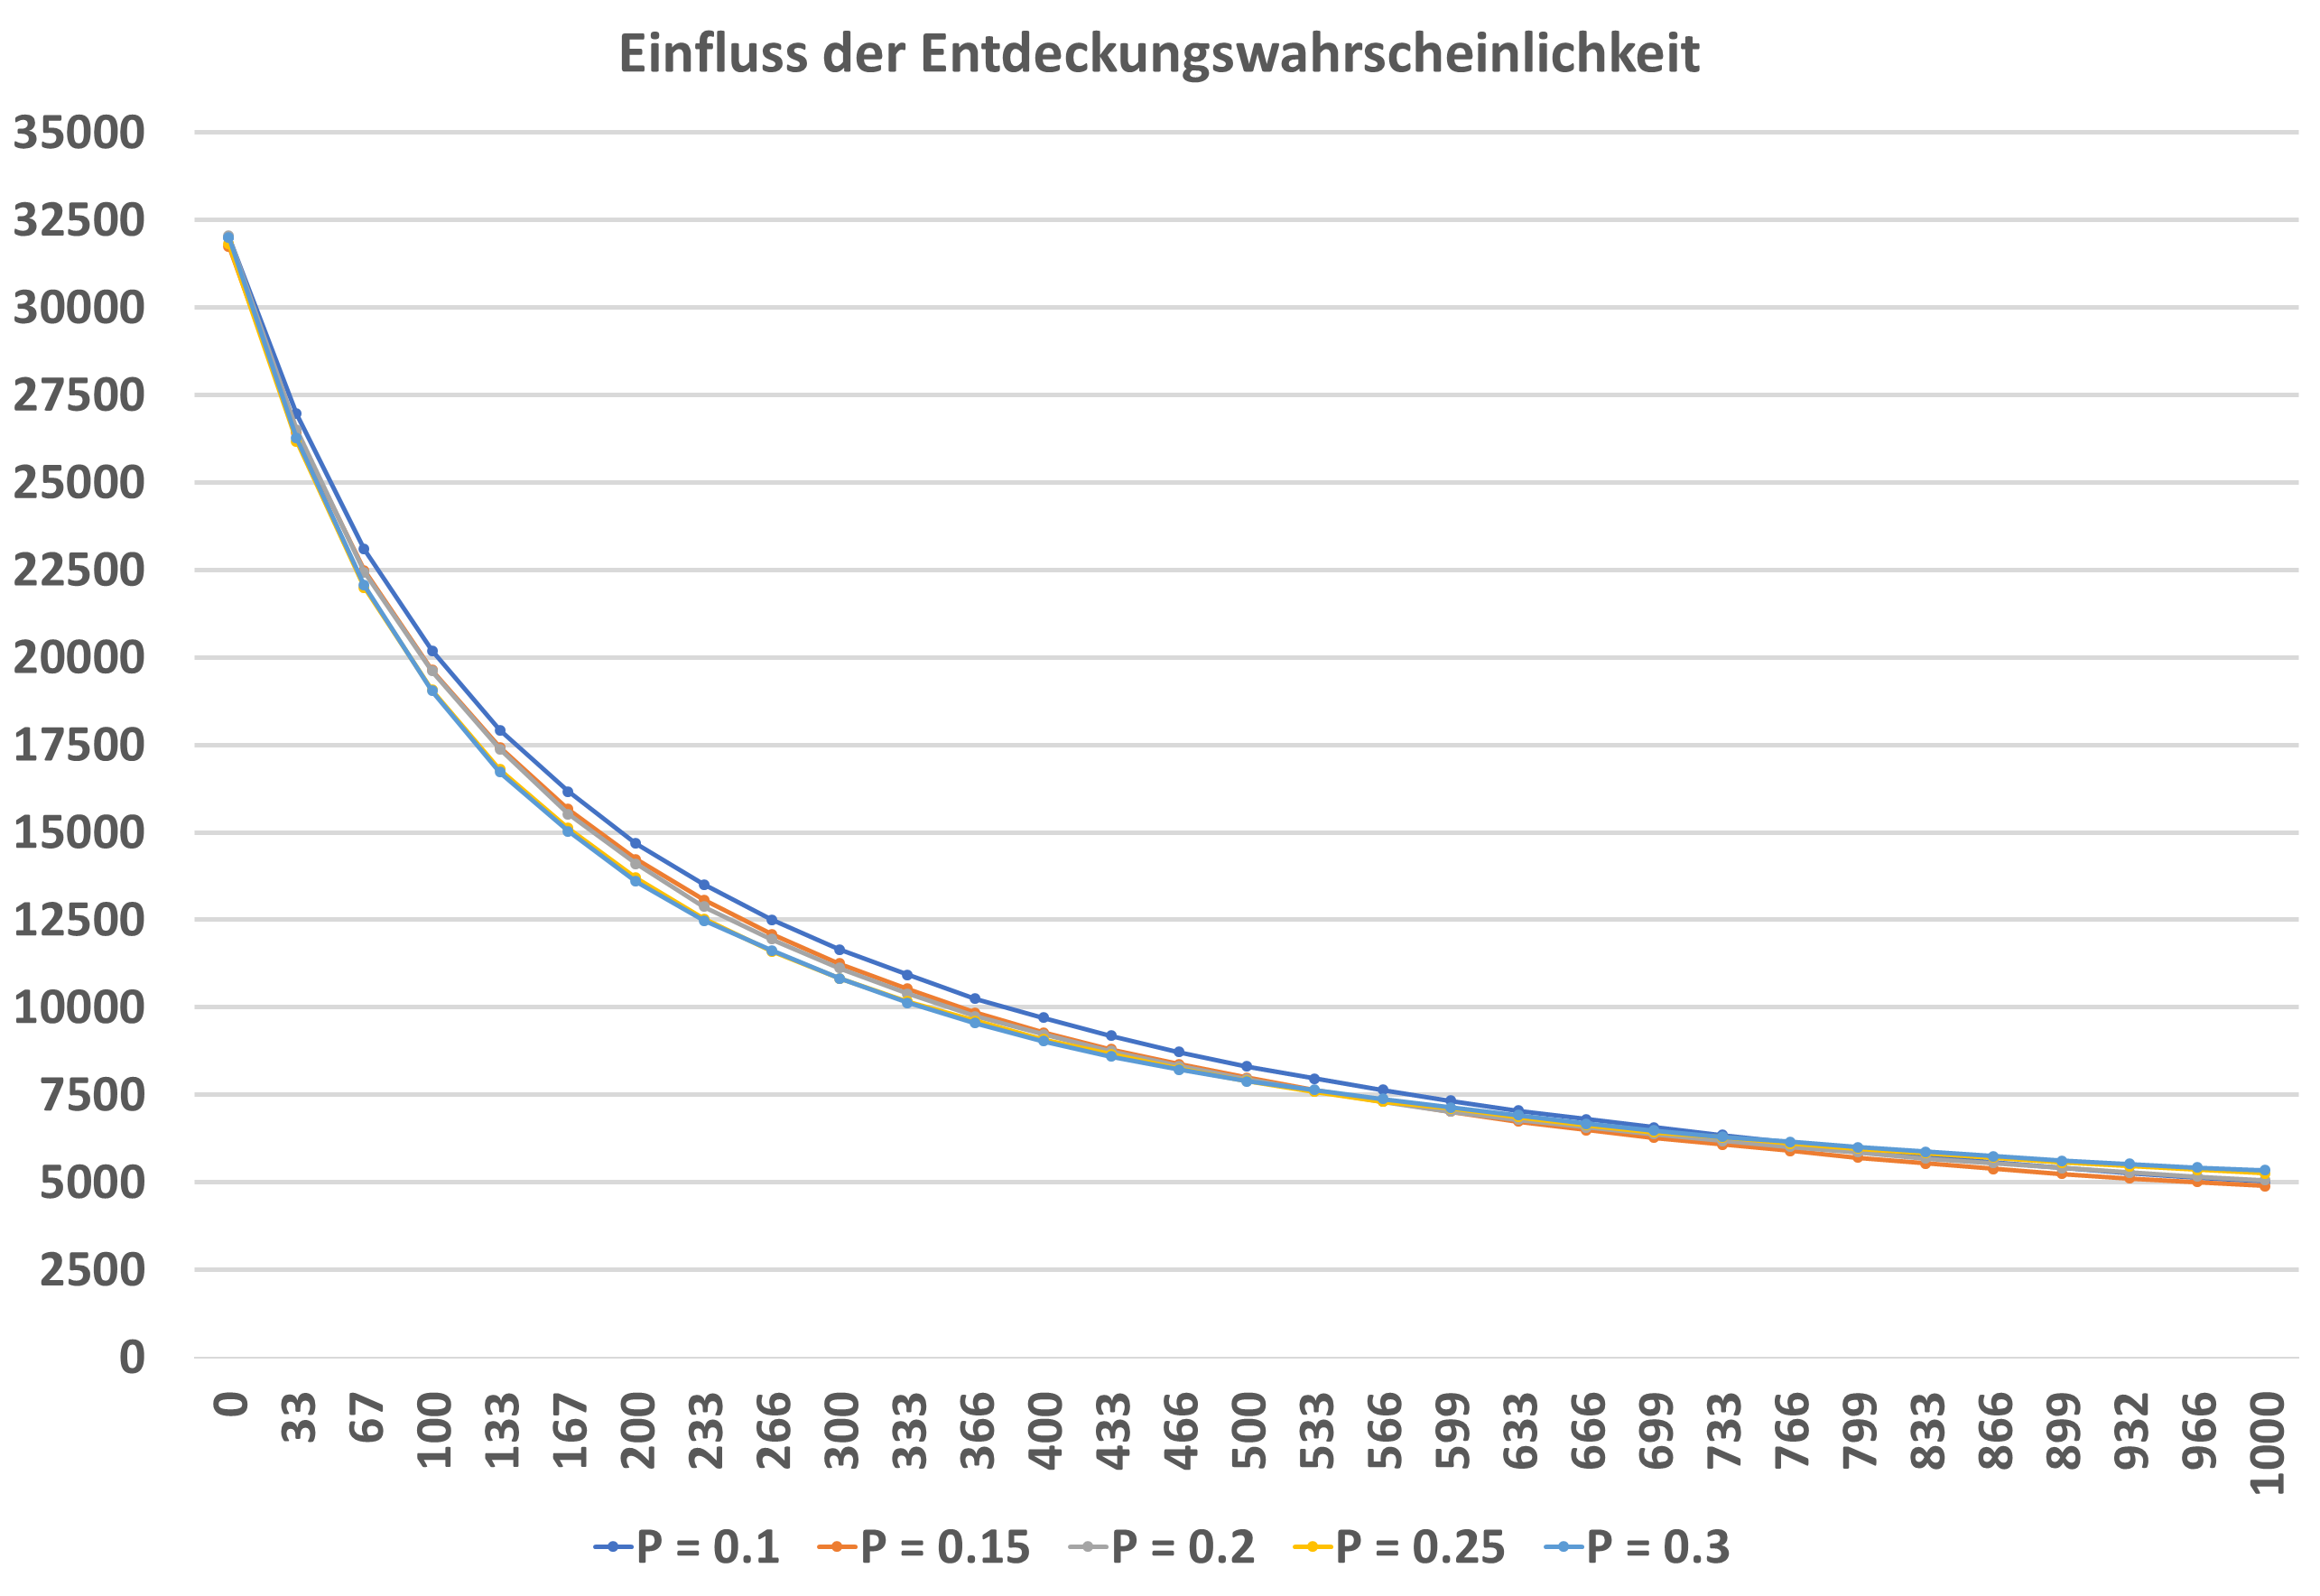
\includegraphics[width=0.8\linewidth]{Entdeckungswahrscheinlichkeit.png}
        \caption{Einfluss des Parameter $P_a$ auf das Ergebnis}
        \label{fig:pa}
      \end{figure}

      Als nächsten wurde der Einfluss der Nester auf das Ergebnis geprüft. Dafür wurden acht Durchläufe mit steigender Anzahl an Nestern von 25 bis 200 
      gemacht. Hierbei wurden eine $P_a$ von 0.15 und 1000 Generationen genutzt. Die Ergebnisse (Abb. \ref{fig:nests}) zeigt, dass mit steigerender Anzahl der Nester wieder
      ein schnelleres Anpassungsverhalten vorliegt, dass aber wiederrum mit ansteigender Anzahl an Generationen verschwindet. Damit hat die Anzahl der Nester auch wieder
      nur einen geringen Einfluss auf die Endqualität des Ergebnisses. Daher setzen wir für weitere Test die Anzahl an Nestern auf 50 fest.
 

      \begin{figure}[H]
        \centering
        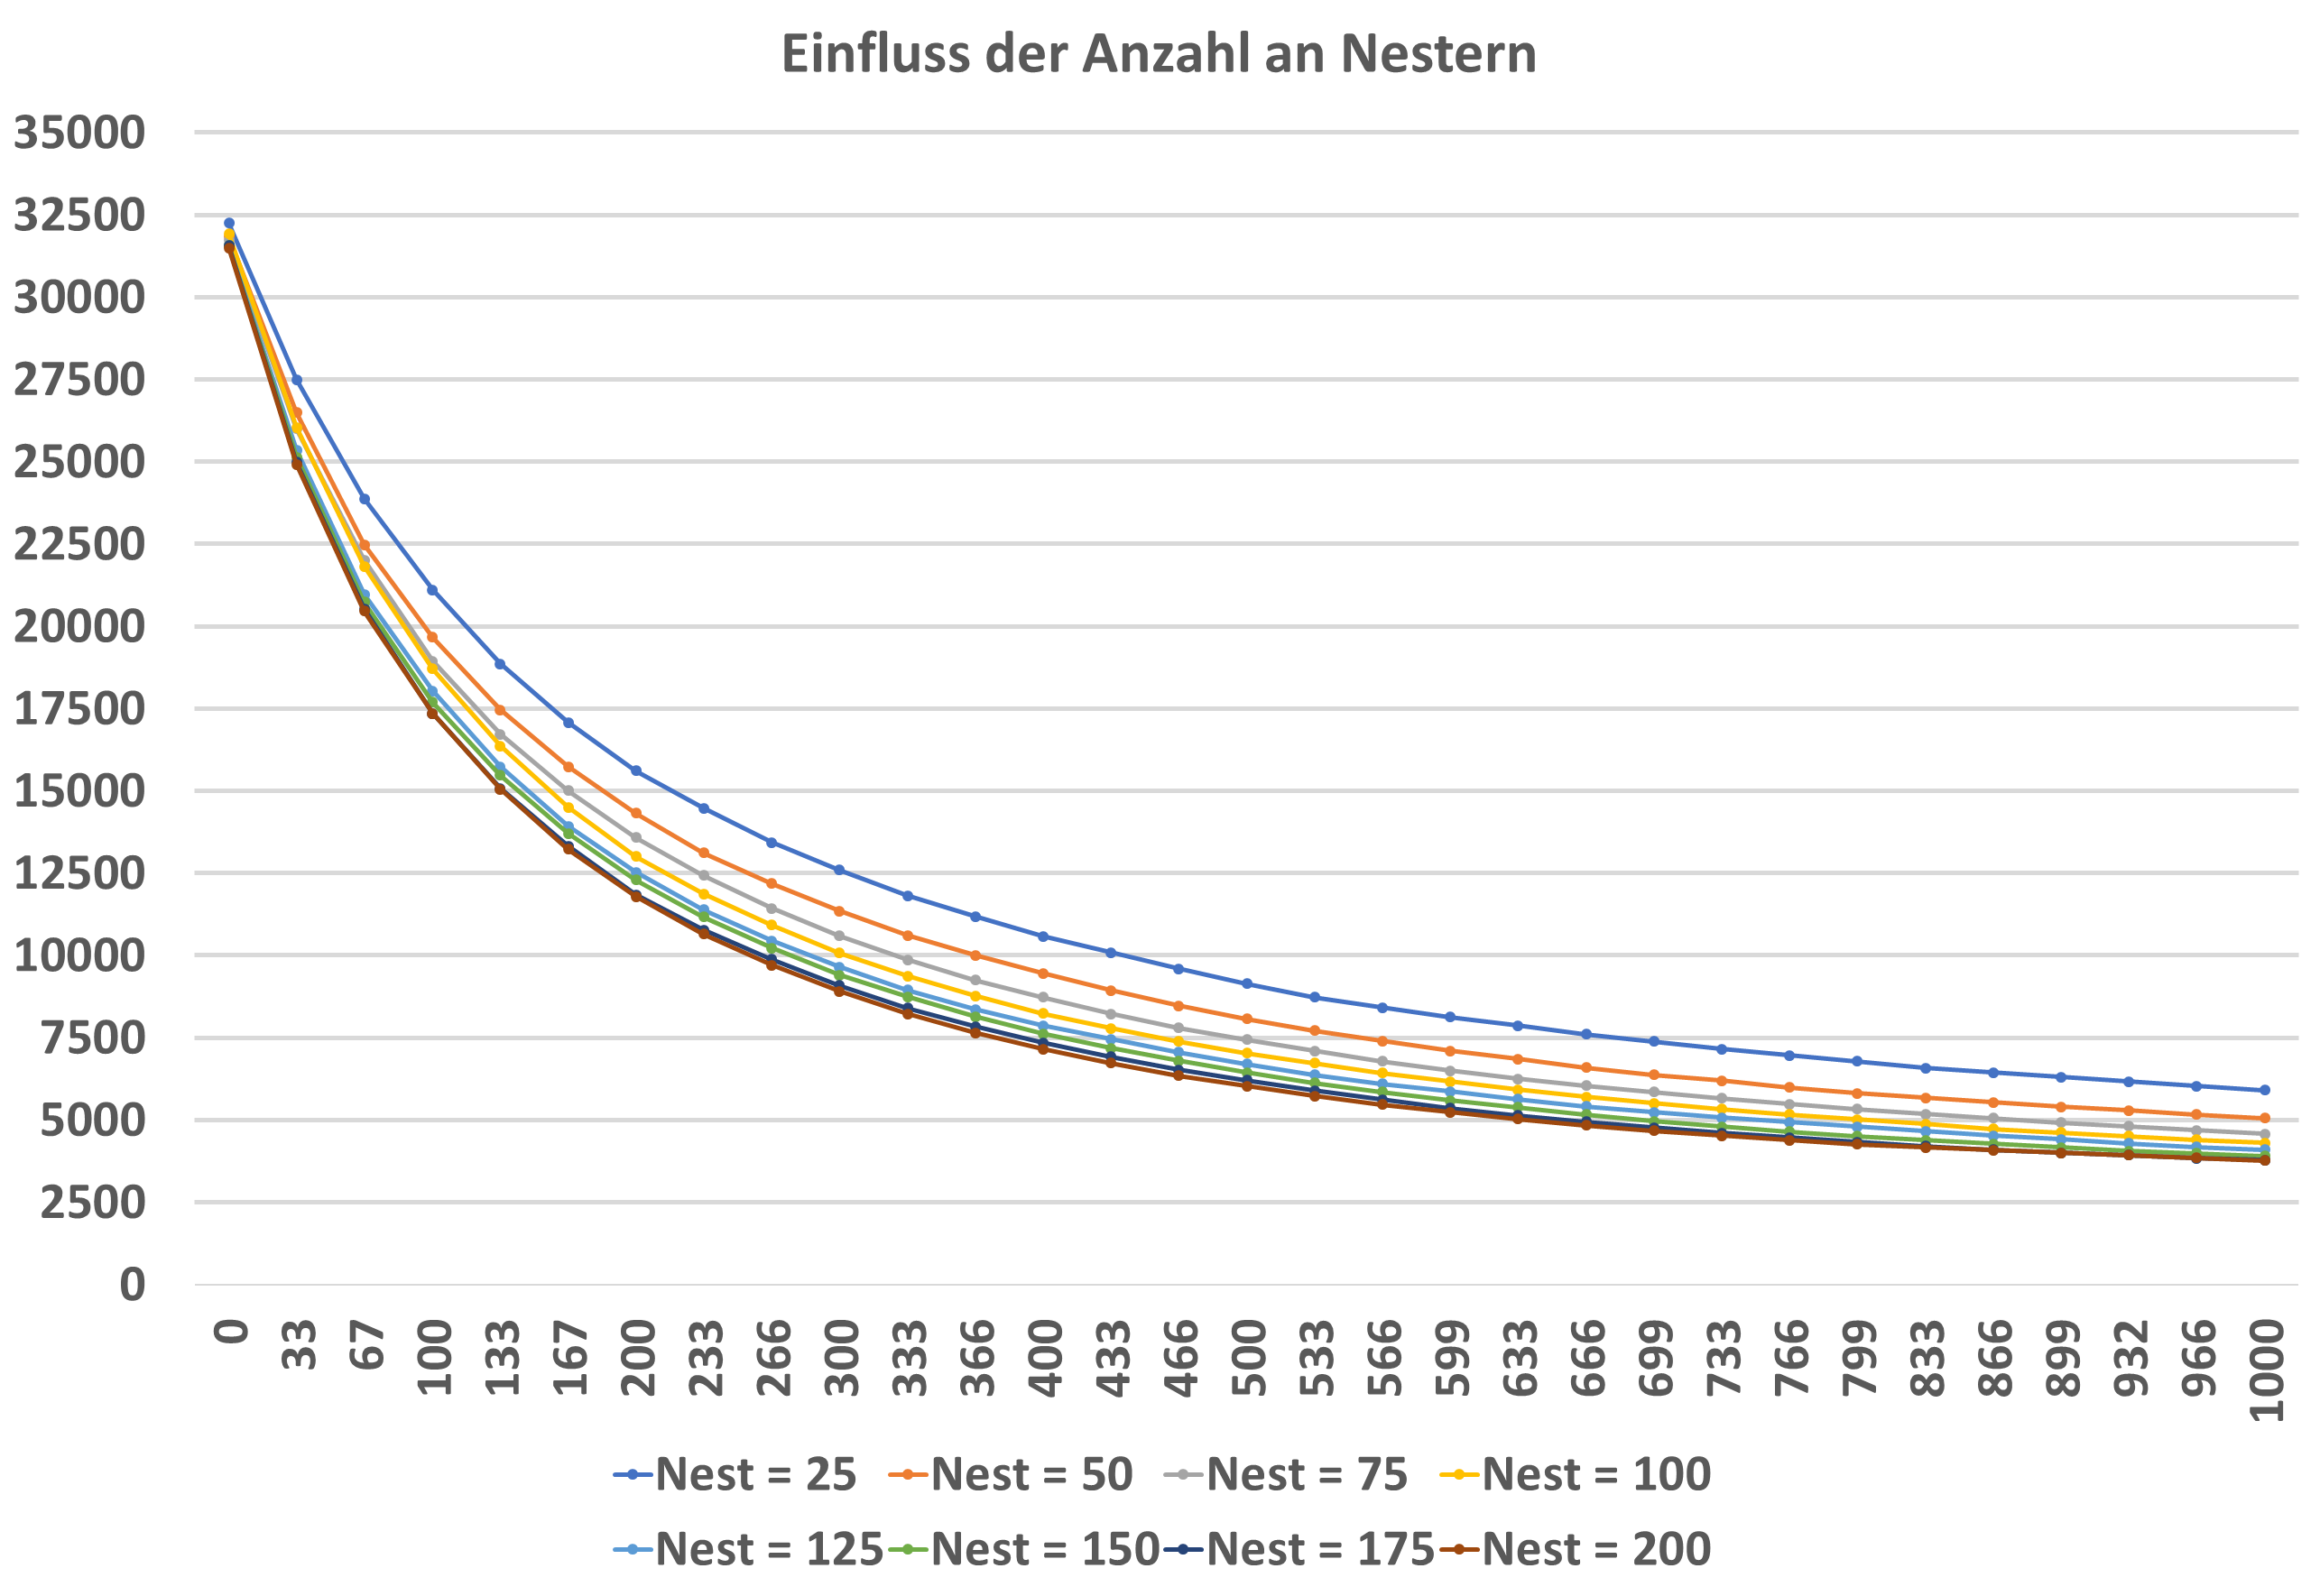
\includegraphics[width=0.8\linewidth]{Nester.png}
        \caption{Einfluss Anzahl der Nester auf das Ergebnis}
        \label{fig:nests}
      \end{figure}

      In Abbildung \ref{fig:generation} ist der Einfluss des Generation Parameters zu erkennen. Für den Durchlauf wurden 50 Nester und eine $P_a$ von 0.15 genutzt. 
      Zu erkennen ist, dass der Algorithmus bis 3400 Iterationen sich langsam immer weiter anpasst. Ab 3400 nimmt diese Kurve immer weiter ab, bis so gut wie keiner Verbesserung
      mehr stattfindet. Diese Schranke lässt sich mittels Anpassung der Anzahl der Nester und des Werte $P_a$ weiter nach links, und somit $<3400$, oder rechts $>3400$ verschieben.
      Generell lässt sich daher sagen, dass mit den von uns gewählten Parametern nur noch geringe Verbesserungen über 4000 Iterationen eintreten.


      \begin{figure}[H]
        \centering
        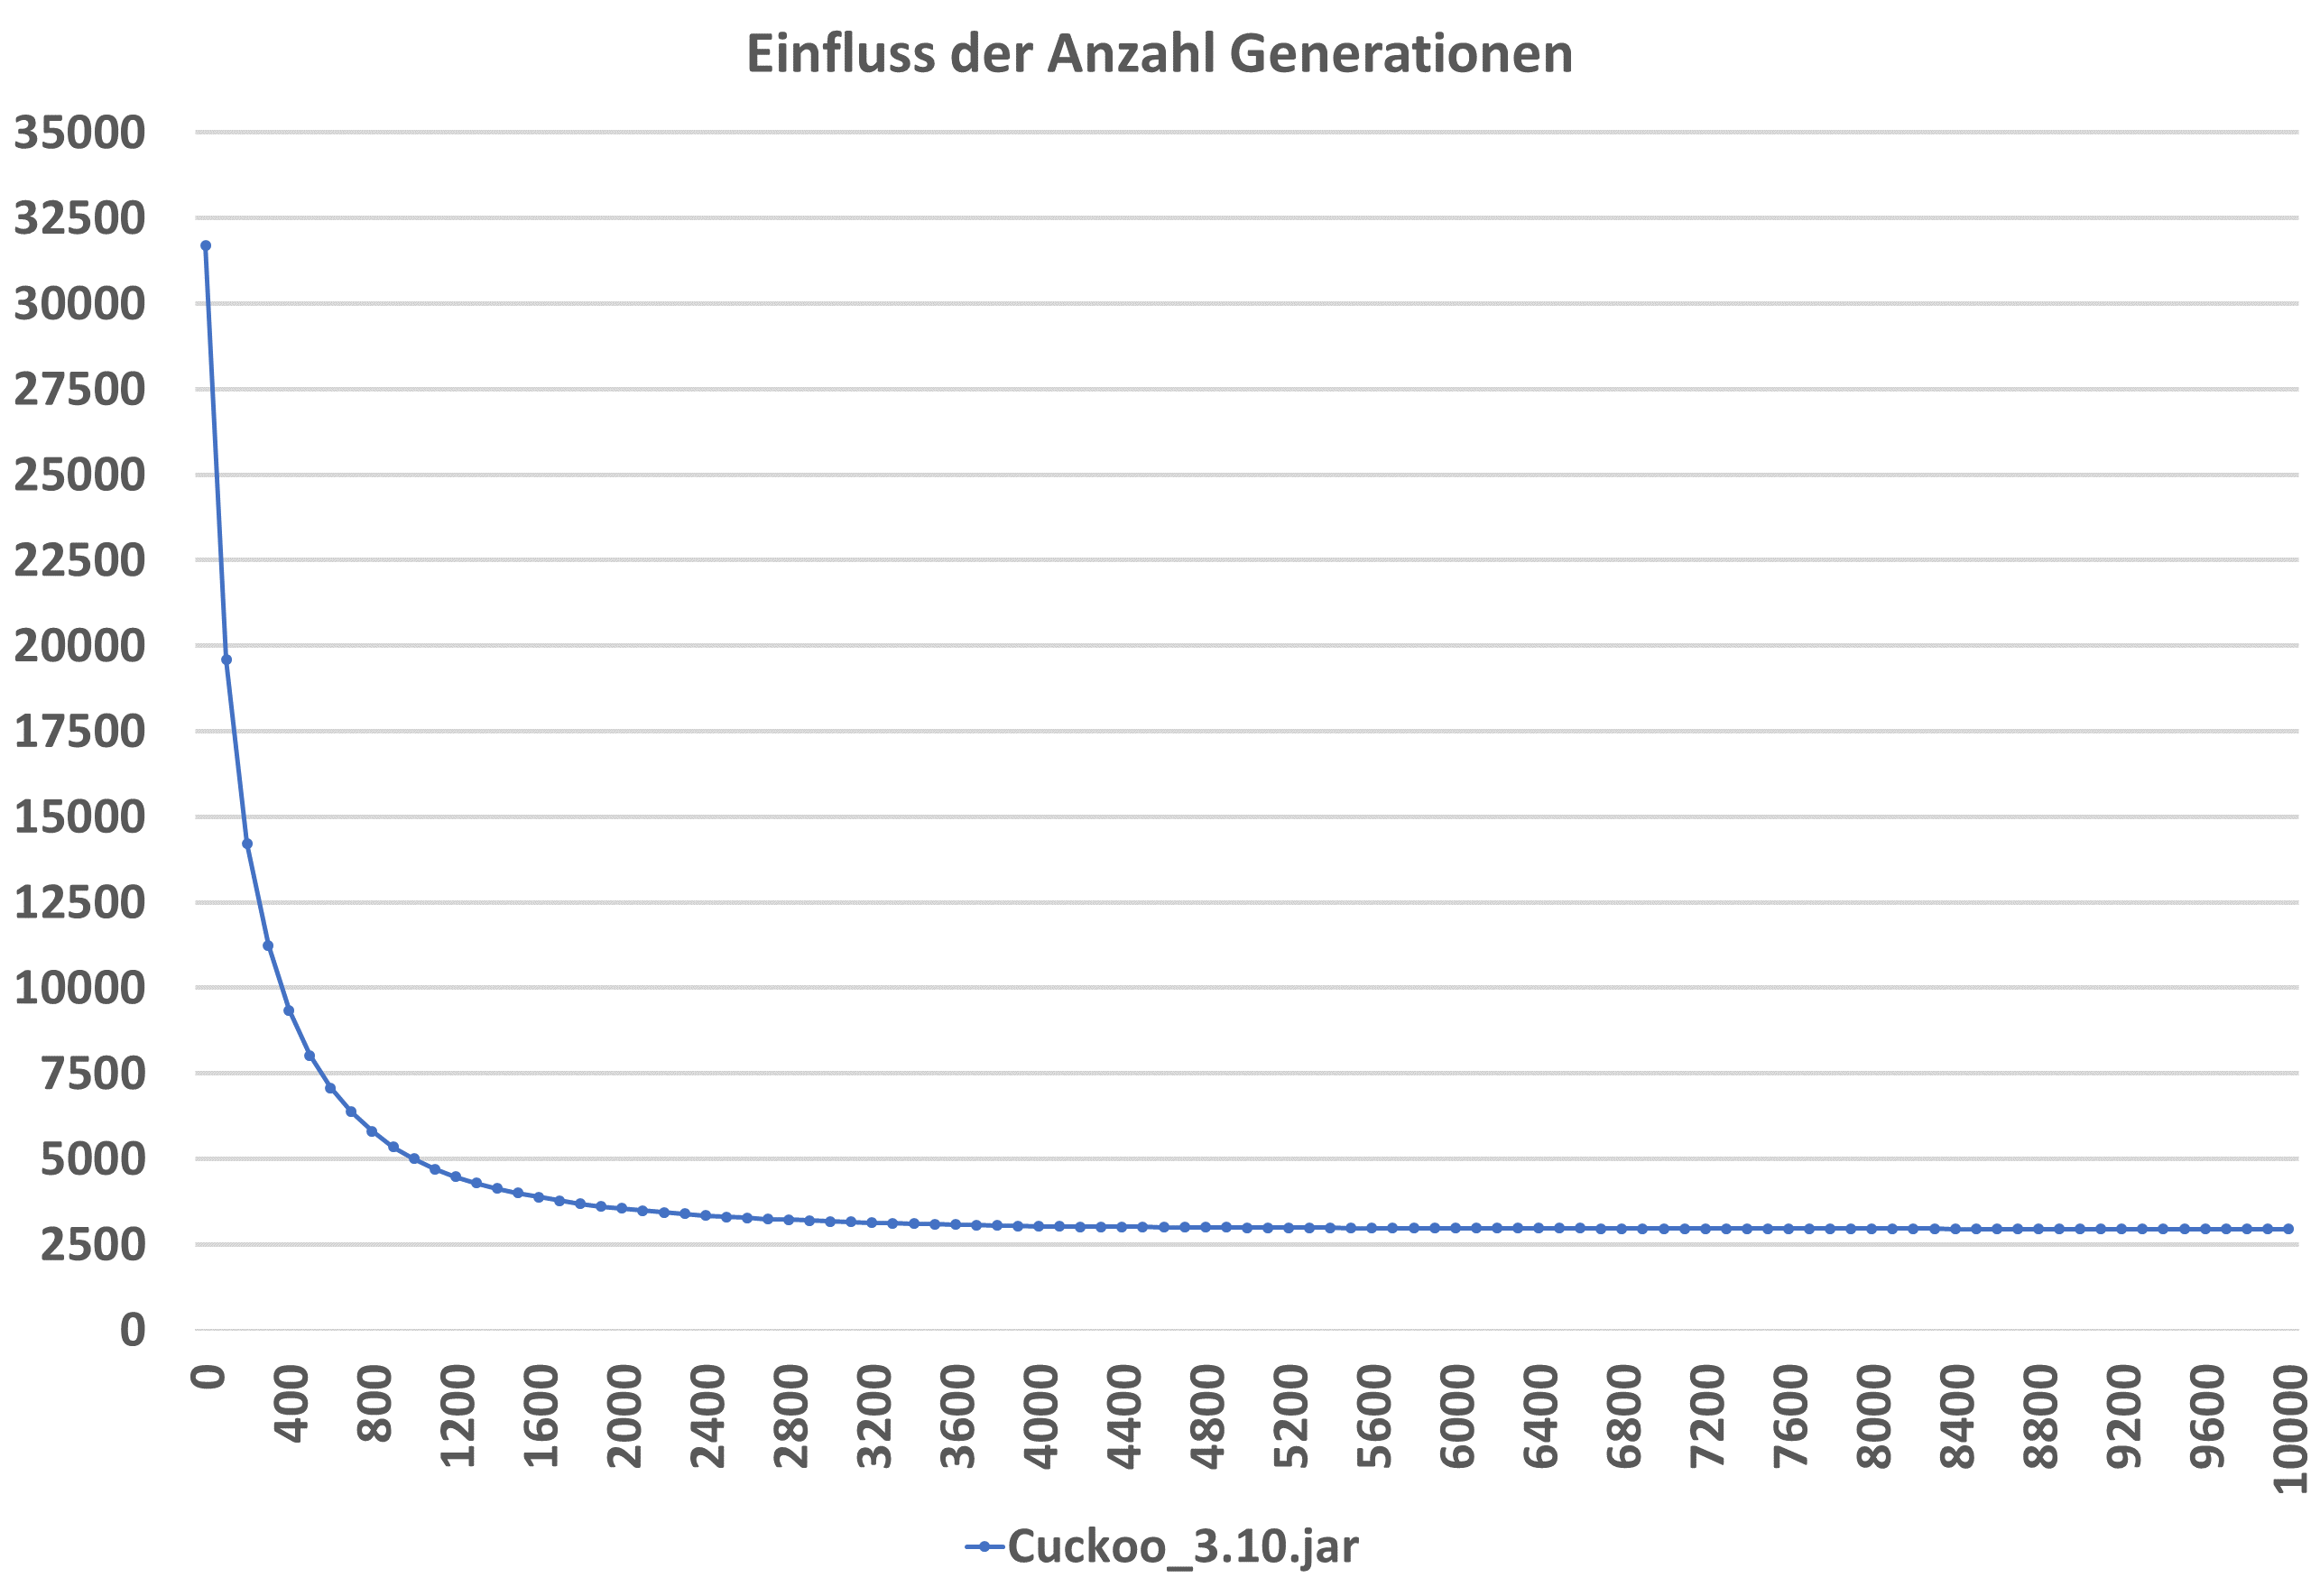
\includegraphics[width=0.8\linewidth]{Generation2.png}
        \caption{Einfluss Anzahl der Generationen auf das Ergebnis}
        \label{fig:generation}
      \end{figure}

      Daher sind unsere Parameter für den Cukoo's Algorithmus:
      \begin{itemize}
        \item $P_a = 0.15$
        \item Nester = 50
        \item Generationen = 4000
      \end{itemize}

    \subsection{Ergebnisse}
      Im folgendem werden das SOP sowie das TSP anhand einiger Beispiele aus der Datensatzsammlung der Uni-Heidelberg
      \footnote{https://wwwproxy.iwr.uni-heidelberg.de/groups/comopt/software/TSPLIB95/} getestet.
      Dabei werden die Parameter aus dem vorherigen Abschnitt genutzt. 
      Die Ergebnisse sind der Mittelwert aus 10 Durchläufe auf dem jeweiligen Datensatz.



      \begin{table}[H]
        \label{table:TSP}
        \centering
        \begin{tabular}{|l|ll|l|l|}
        \hline
            Datensatz & \multicolumn{1}{l|}{Start} & End  & Best & $\sim$\%-Abweichung \\ \hline
            berlin52.tsp  & \multicolumn{1}{l|}{26174} & 7949 & 7542 & 0,05       \\ \hline
            ch130.tsp  & \multicolumn{1}{l|}{42378} & 6683 & 6110 & 0,09       \\ \hline
            a280.tsp  & \multicolumn{1}{l|}{31874} & 2974 & 2579 & 0,15       \\ \hline
            d493.tsp  & \multicolumn{1}{l|}{430752} & 43334 & 35003 & 0,23       \\ \hline
            d1291.tsp  & \multicolumn{1}{l|}{1682530} & 222502 & 50801 & 3,38       \\ \hline
        \end{tabular}
        \caption{Ergebnisse TSP}
      \end{table}

      Unser Algorithmus performt bei kleinen TSP's gut, hingegen mit steigender Komplexität des TSP's steigt die Abweichung zum Optimalen enorm an. 
    

      \begin{table}[h]
        \label{table:SOP}
        \centering
        \begin{tabular}{|l|ll|l|l|}
        \hline
            Datensatz & \multicolumn{1}{l|}{Start} & End  & Best & $\sim$ \%-Abweichung \\ \hline
            br17.10  & \multicolumn{1}{l|}{119} & 55 & 55 & 0,00       \\ \hline
            ESC25  & \multicolumn{1}{l|}{9477} & 2881 & 1681 & 0,71       \\ \hline
            ESC63  & \multicolumn{1}{l|}{228} & 96 & 62 & 0,59       \\ \hline
            rgb174a  & \multicolumn{1}{l|}{2940} & 2342 & 2053 & 0,14       \\ \hline
            rgb358a  & \multicolumn{1}{l|}{6626} & 4292 & [2518, 2758] & [0,7 - 0,54]       \\ \hline
        \end{tabular}
        \caption{Ergebnisse SOP}
      \end{table}

      Das SOP ist ein komplexeres Problem als das TSP, wodurch sich die Schwierigkeit nicht direkt anhand der Anzahl an Knoten ablesen lässt.
      Daher schwankt hier die Güte des Cuckoo's Algorithmus zwischen größeren und kleineren SOP's stark. 

  \section{Fazit}
    Der Cuckoo's Algorithmus überzeugt durch seine geringe Komplexität, 
    guten Laufzeit, anschaulichen Ergebnissen und Robustheit gegen Änderungen. 
    Die Stärke des Algorithmus ist daher auch gleichzeitig seine Schwäche. Durch den Verzicht 
    auf weitere Metriken, sind Anpassung und damit Einwirkungen auf den Ablauf des Algorithmus schwierig. 
    Der Cuckoo's Algorithmus eignet sich daher gut für kleinere Optimierungsprobleme für die schnell ein relativ 
    gutes Ergebnis gefunden werden muss. Für perfekte Resultate oder größere Probleme ist die Anpassungsmöglichkeit 
    nicht gegeben, weshalb auf komplexere Algorithmen zurückgegriffen werden sollte. 


  \begin{thebibliography}{00}
  \bibitem{b1} Yang, X.Ss, Deb, S.: Cuckoo search via lévy flights. In: Nature and biologically inspired computing, 2009. NaBIC 2009. World congress on, IEEE, pp 210–214, (2009) .
  \bibitem{b2} Lawler, E.L., Lenstra, J.K., Kan, A.R., Shmoys, D.B.: The traveling salesman problem: a guided tour of combinatorial optimization, vol 3. Wiley, New York (1985) .
  \bibitem{b3} Gutin, G., Punnen, A.P.: The traveling salesman problem and its variations, vol 12. Springer, New York (2002).
  \bibitem{b4} Pavlyukevich, I.: Lévy flights, non-local search and simulated annealing, J. Computational Physics, 226, 1830-1844 (2007).
  \bibitem{b5} Pavlyukevich, I.: Cooling down Lévy flights, J. Phys. A:Math. Theor., 40, 12299-12313 (2007).
  \bibitem{b6} Reynolds, A.M., Frye, M.A.: Free-flight odor tracking in Drosophila is consistent with an optimal intermittent scale-free search, PLoS One, 2, e354 (2007).
  \bibitem{b7} Yang, X.S.: Cuckoo Search and Firefly Algorithm: Theory and Applications, chap. Cuckoo Search and Firefly: Overview and Analysis, pp. 1-26. Springer Publishing Company, Incorporated (2013).
  \bibitem{b8} Leccardi, M.: Comparison of three algorithms for Lévy noise generation. In: Proceedings of Fifth EUROMECH Nonlinear Dynamics Conference, Mini Symposium on Fractional Derivates and their Applications (2005).
  \bibitem{b9} Quaarab, A., Ahiod, B., Yang, X.S.: Discrete cuckoo search algorithm for the travelling salesman problem. Neural Comput and Applic (2014) 24:1659–1669, DOI 10.1007/s00521-013-1402-2.
  \bibitem{b10} Croes, G.A.: A Method for Solving Traveling-Salesman Problems. Operation Research, 6, 791-812, (1958). 
  \bibitem{b11} Martin, O., Otto, S.W., Felten, E.W.: Large-Step Markov Chains for the traveling salesman problem. Complex Syst. 5(3), 299-326 (1991).
  \bibitem{b12} https://www.iwr.uni-heidelberg.de/groups/comopt/software/TSPLIB95/ Zuletzt aufgerufen: 30.01.2019
      

  \end{thebibliography}


\end{document}
